\ylDisplay{Kujutise kiirus} % Ülesande nimi
{koit Timpmann} % Autor
{lõppvoor} % Voor
{2019} % Aasta
{P 5} % Ülesande nr.
{3} % Raskustase
{
% Teema: Valgusõpetus
\ifStatement
Punkt $A$ liigub kiirusega $v = 2$ cm/s risti läätse optilise peateljega. Kui suure kiirusega liigub selle punkti kujutis? Punkti $A$ projektsioon optilisele peateljele asub läätse keskpunktist $a = 15$ cm kaugusel ja läätse fookuskaugus $f = 10$ cm.
\begin{center}
	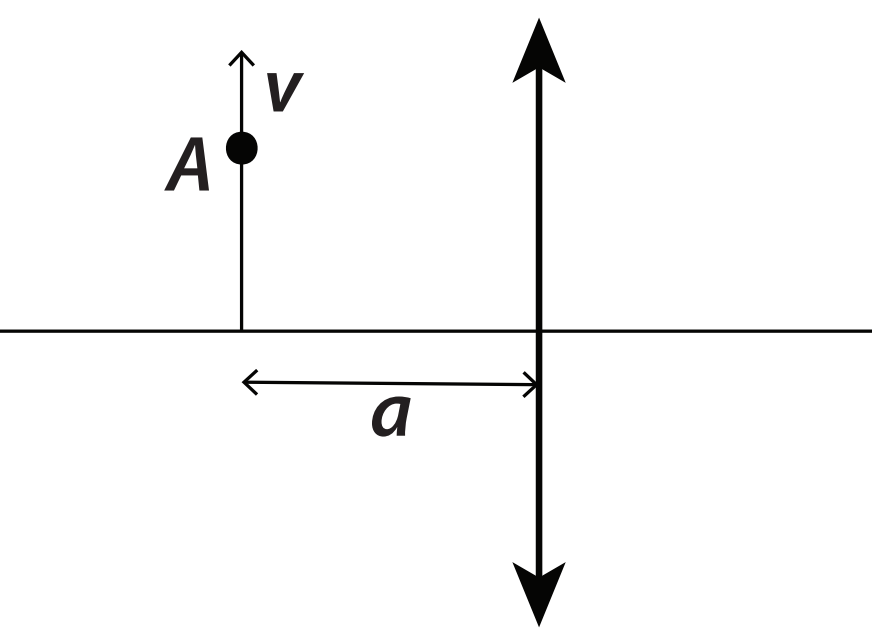
\includegraphics[width=0.5\linewidth]{2019-v3p-05-yl.PNG}
\end{center}
\fi
\ifHint
Ülesande lahendamiseks konstrueeri joonis ning kasuta sarnaste kolmnurkade seoseid.
\fi
\ifSolution
\begin{center}
	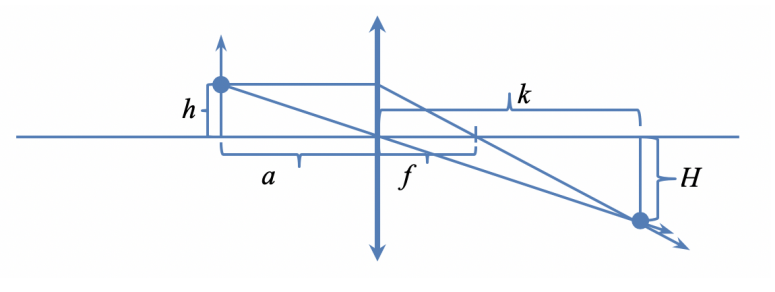
\includegraphics[width=0.5\linewidth]{2019-v3p-05-lah.PNG}
\end{center}
Oletame, et punkt $A$ asub kaugusel $h$ läätse optilisest peateljest. Punkti $A$ kujutis asub sel juhul kaugusel $H$ optilisest peateljest. Sarnastest kolmnurkadest saame avaldada seosed:
\begin{center}
$\cfrac{h}{a} = \cfrac{H}{k}$ ja $\cfrac{h}{f} = \cfrac{H}{k - f}$ .
\end{center}
Avaldame esimesest seosest $H$ ja asendame selle teise seosesse,
\begin{center}
$H = \cfrac{hk}{a}$ ning $\cfrac{h}{f} = \cfrac{hk}{a(k - f)}$, 
\end{center}
millest
\begin{center}
$k = \cfrac{af}{a - f} = 30$ cm 
\end{center}
Punkt $A$ liigub kiirusega $v$ optilisest peateljest eemale. Seega ajavahemiku $t$ pärast on punkti $A$ kaugus optilisest peateljest $h + vt$ ehk $h + s$. Ka kujutis liigub optilisest peateljest eemale, kuid kiirusega $v_1$. Seega on kujutise kaugus sama ajavahemiku pärast optilisest peateljest $H + v_1t$ ehk  $H + S$. Sarnastest kolmnurkadest saame, et
\begin{center}
$\cfrac{h}{a} = \cfrac{H}{k}$ , 
\end{center}
millest
\begin{center}
$H = \cfrac{hk}{a}$
\end{center}
ning kui punkt on liikunud aja $t$ võrra 
\begin{center}
$\cfrac {h + s}{a} = \cfrac {H + S}{k}$. 
\end{center}
Asendame $H$ ja saame, et 
\begin{center}
$S = \cfrac {sk}{a}$ . 
\end{center}
Võtame ajavahemikuks $1$ s ning saame, et $S = 4$ cm, mis teeb kujutise kiiruseks $4$ cm/s. 
\fi
}